% --------------------------------------------------------------------------
% Lane D contribution to the 4-6 page comment/extension note.
% Sections: III (reproduction), IV (infeasible region), V (floor does not
% order the frontier). Merge target:.work3/note_skeleton.md sections
% 1/2/3/7/8. Wording discipline: comment / extension / clarifying remark.
% Every number below carries its provenance in the reproduction map
% (Appendix~\ref{app:repro}); the lane-marker macro has been dropped for
% submission, the source table is kept in the repro package.
% --------------------------------------------------------------------------

\section{Reproducing the published rate--cost frontiers}
\label{sec:repro}

The reference example of \cite{refpaper} is a four-state plant with
$|\operatorname{eig}(A)|=\{1.7124,\,1.3127,\,0.2848\pm0.6984i\}$, process noise
covariance $W\succ0$, and the weighting $\Theta$ and offset $j_c$ of
\eqref{eq:cost}, which evaluate to $j_c=31.4833$.

Two scalar anchors are reproduced before any of our own claims are made:

\begin{enumerate}
 \item the minimum stabilizing rate $\sum_{|\lambda_u|>1}\log_2|\lambda_u|
 = 1.168575$ bits/sample, against the value $1.169$ printed in the
 published figure;
 \item the four curves of the published figure (\cite[Fig.~1]{refpaper}) ---
 three task-restricted frontiers and the
 unrestricted reference ---, digitised from the
 vector artwork (frame pixels $x\in[121,1924]$, $y\in[52,1238]$,
 $D\in[40,90]$, $I\in[1,5]$; $1$\,px~$=0.0278$ in $D$; calibration
 ambiguity between frame edge and grid line $\pm0.09$, plus the
 read-off-convention spread of Table~\ref{tab:red}).
\end{enumerate}

The digitised curves span $D\in[46.99,89.83]$, $I\in[1.543,4.921]$ (red,
$r=2$), $D\in[40.08,89.78]$, $I\in[1.535,3.498]$ (blue, $r=3$),
$D\in[40.08,89.89]$, $I\in[1.516,3.263]$ (magenta, $r=4$) and
$D\in[40.83,89.14]$, $I\in[1.170,3.125]$ (the unrestricted curve); the raw
per-pixel-column lists are in \texttt{data/fig1\_digitized.csv} ($5760$ rows).

\begin{remark}[calibre]
\label{rmk:calibre}
There are two natural ways to evaluate the frontier of a task-restricted sensor
with admissible range $V$: the \emph{ray} calibre, in which the information
matrix injected on $V$ is held isotropic, $S=vP_V$, and the scalar $v$ is
swept; and the \emph{cone} calibre,
in which $S\in\mathcal K_F$ ranges over the whole admissible cone,
$S=U_F M U_F^{\top}$ with $M\succeq0$ arbitrary, i.e.\ the closure of
$\mathcal K_F$ is used and rank-deficient $S$ (a channel switched off entirely)
is admissible. 
\end{remark}

\begin{table}[h]
 \centering\caption{Frontier of the published $r=2$ sensor, both calibres,
 against the digitised red curve. $\Delta$ is in units of $D$.}
 \label{tab:red}
 \begin{tabularx}{\columnwidth}{Xlrl}
 \hline
 target $I$ & digitised $D$ & cone $\big(\Delta_{\rm cone}\big)$ &
 ray $S=vP_V$ \\
 \hline
 $2.00$ & $62.902\,\pm0.021$ & $62.8975\ (-0.005)$ & $79.3018$ \\
 $2.50$ & $54.311\,\pm0.014$ & $54.2924\ (-0.019)$ & $63.3839$ \\
 $3.00$ & $50.651\,\pm0.003$ & $50.6023\ (-0.049)$ & $56.2321$ \\
 $4.00$ & $47.978\,\pm0.007$ & $47.9396\ (-0.038)$ & $50.2372$ \\
 $4.90$ & $47.040\,\pm0.006$ & $47.1006\ (+0.061)$ & $48.1475$ \\
 \hline
 \end{tabularx}
 \\[1pt]{\scriptsize The $\pm$ is the spread over four read-off conventions
 (nearest pixel column, two rate windows, polyline crossing), which is needed
 because the curve is steep at the low-rate end: between $I=1.95$ and $2.05$
 the red curve moves by $2.6$ units of $D$, $94$ pixels. All four conventions
 are printed by \texttt{repro/readoff.py}.}
\end{table}

Two things must be kept apart, and only the second one carries the argument.
The cone residuals are small and of both signs: $-0.005$, $-0.019$, $-0.049$,
$-0.038$, $+0.061$, i.e.\ at most $2.2$ pixels and inside the $\pm0.09$
calibration band quoted above. The cone calibre is therefore
\emph{consistent} with the published curve at all five anchors and nothing more
--- no sign is resolvable, and we do not ask more of the artwork than that. What
the artwork does resolve is the other comparison: every ray value lies
\emph{above} the published curve by $1.11$--$16.40$, i.e.\ by $40$ to $590$
pixels, at least $18$ times the largest cone residual. Being above is not
itself a contradiction --- a suboptimal family may well cost more --- but it
does exclude identity: on the same plant, the same axis and the same sensor, the
published curve is better than anything the isotropic family achieves. We
therefore read the published figure as the \emph{cone} optimum of the paper's
own Theorem~1 set, with the
maximiser sitting on or near the rank-deficient boundary (optimal second-channel weight
$\rho^{\star}=0$ for $I\le3$ and $\rho^{\star}\le0.1$ at the two highest anchors,
optimal in-plane angle $\theta^{\star}\in[128^{\circ},138^{\circ}]$),
and not as any isotropic-noise subfamily. 

For the unrestricted curve the two calibres coincide to within the read-off
spread: the free-cone optimum is $58.1931$ at $I=2$ against
$58.040\,\pm0.159$ digitised, and $47.756$ at $I=2.5$ against
$47.758\,\pm0.077$. The $I=2$ residual is larger than the red-curve ones only
because the unrestricted curve is steeper there; no sign is readable at that
point, and none is claimed. 

\begin{remark}[one curve we cannot place]
\label{rmk:blue}
The blue ($r=3$) curve is not reproduced. Over the Schur-tail $3$-plane the cone
optimum is $59.5611$ at $I=2$, and the digitised curve sits $0.78$ above it
($60.344\,\pm0.265$) --- the admissible direction. At $I=3$ the same cone optimum
is $45.4537$ while the digitised curve is at $43.711\,\pm0.007$, i.e.\ $1.74$
\emph{below} the best design of that plane: $250$ times the read-off spread and
$19$ times the $\pm0.09$ calibration band, so this is not a measurement artefact.
The plane's minimum is obtained by multistart local search, so $45.4537$ is an
upper bound on what that plane can deliver and the exclusion is stated relative
to that bound. A certified lower bound would make it absolute; the best one
available, \eqref{eq:cond} evaluated on that plane (Section~\ref{sec:waterfill},
where the frontier-wide step needs a monotonicity that is \emph{false}
(falsified in the cone: a closed-form rank-one counterexample and $115$
reachable counterexamples), so \eqref{eq:cond} is quoted only as its value at
the wall prior), is $41.485$ at $I=3$, i.e.\ $2.23$ \emph{below} the digitised value, so
this note does not make the exclusion absolute.
The point itself is feasible globally, since the free optimum at $I=3$ is
$42.040<43.711$; so the published $r=3$ curve must use a different
$3$-dimensional admissible subspace than the one we assumed. We do not attempt
to fit it in this note. 
\end{remark}

\section{The infeasible region, and what the published figure can show}
\label{sec:infeasible}

For an admissible subspace $V=\operatorname{range}(S)$, with $P_V$ the orthogonal
projector onto $V$, define
\begin{equation}
 D_{\min}(V)\;=\;j_c+\Phi_0(V),\qquad
 \Phi_0(V)=\inf_{\tau>0}\operatorname{tr}\!\big(\Theta P_m(\tau P_V)\big),
\end{equation}
the zero-measurement-noise limiting cost, reached as the information matrix
scales to infinity along $V$. Three independent evaluations (information-form
fixed point, singular DARE, filter DARE
$\texttt{sdare}(A^{\top},F^{\top},W,V)$) agree to $1.3\times10^{-3}$ on the
anchors $V=\operatorname{range}(F_2^{\top})$, $D_{\min}=46.1231$, and
$V=\operatorname{span}\{\theta_1,\theta_2\}$, $D_{\min}=32.2751$.


\begin{proposition}[shape of the infeasible region]
\label{pr:region}
Fix $V$ with $\dim V\ge1$ and let the plant pair $(A,\,V)$ be detectable. Then
along the ray $\{\tau P_V\}$ the rate is unbounded,
$\lim_{\tau\to\infty} I(\tau P_V)=\infty$, while the cost decreases to the
finite limit $D_{\min}(V)$. Hence
\begin{itemize}
 \item[(i)] $\{D<D_{\min}(V)\}$ is infeasible at \emph{every} rate: the wall is
 a horizontal asymptote of the frontier, not a point on it;
 \item[(ii)] if the pair is not detectable, no $\tau$ yields a stationary
 error covariance, and the whole ray is infeasible
 ($D_{\min}(V)=+\infty$);
 \item[(iii)] the frontier of a subspace with a lower wall does not lie below
 the frontier of a subspace with a higher wall (Section~\ref{sec:nofactor}).
\end{itemize}
\end{proposition}

\begin{proof}[Proof sketch]
(i) $\det P_m(\tau P_V)$ shrinks as $1/\tau$ on $V$ and stays bounded away from
zero on a complement only if $V$ is not detectable; the ratio
$\det(A P_m A^{\top}+W)/\det P_m$ therefore diverges logarithmically while
$\operatorname{tr}(\Theta P_m)$ converges monotonically to the zero-noise limit,
which is exactly $\Phi_0(V)$. Concretely, $r=\dim V$ directions carry the
$\tau^{-1}$ factor, so $I(\tau P_V)=\tfrac r2\log_2\tau+O(1)$ and the wall is
approached geometrically,
\begin{equation}
 D(I)-D_{\min}(V)\;\approx\;C(V)\,2^{-2I/r}.
\label{eq:decay}
\end{equation}
(ii) is the standard equivalence between convergence of the information-form
recursion and detectability; the Schur-tail-$1$ row of Table~\ref{tab:wall} is
that case observed: one scalar measurement cannot cover both unstable modes
($|\operatorname{eig}(A)|=\{1.7124,1.3127,\dots\}$).
\end{proof}

\begin{remark}[the predicted slope, measured]
\label{rmk:slope}
On the semi-logarithmic axes of Fig.~\ref{fig:wall}, Eq.~\eqref{eq:decay} says
the asymptotic slope is $-2\log_{10}2/r$, i.e.\ $-0.6021$, $-0.3010$, $-0.2007$
per bit for $\dim V=1,2,3$. Least-squares slopes over the decade of rate
$I\in[12,20]$ (for $\dim V=1$, over $I\in[6,12]$, where the gap has not yet left
the axis) give $-0.6022$, $-0.3010$ and $-0.3010$, $-0.2017$ and $-0.2018$: the
two $2$-dimensional families and the two $3$-dimensional families agree with
each other to four digits, and with \eqref{eq:decay} to within $0.5\%$, with no
fitted constant and no family-dependent exponent.

\end{remark}

\begin{remark}[the other end of the same curve is published]
\label{rmk:dual}
Proposition~\ref{pr:region}(i) is the cost-side asymptote. The rate-side one,
$I\to\sum_{|\lambda_i(A)|>1}\log_2|\lambda_i(A)|$ as the cost budget grows, is
already printed for a restricted observation matrix whose unobservable subspace
contains unstable modes \cite[Sec.~IV-A, Fig.~3]{sabag2021reducing}, on this very
plant and with this very constant. Nothing in Proposition~\ref{pr:region} or
Eq.~\eqref{eq:decay} is claimed for that end of the frontier: what we add is the
cost-side wall as a function of $\operatorname{range}(S)$ alone, the measured
slope $-2\log_{10}2/r$ of its approach, and the fact that it does not order the
frontiers (Section~\ref{sec:nofactor}).
\end{remark}

Table~\ref{tab:wall} and Fig.~\ref{fig:wall} measure the approach to the wall for
five admissible subspaces of the published plant, sweeping the ray
$S=vP_V$, $v\in[10^{-3},10^{12}]$.

\begin{table}[h]
 \centering\caption{Horizontal asymptotes: five admissible subspaces $V$ of
 the published plant, each swept along its own ray, and how large a rate the
 published window would need.}
 \label{tab:wall}
 \begin{tabularx}{\columnwidth}{Xcccc}
 \hline
 family & $D_{\min}(V)$ & gap at $I\approx5$ &
 $I$ at $1\%$ & $I$ at $0.1\%$ \\
 \hline
 Schur tail $2$ & $46.1231$ & $4.33\%$ & $7.1$ & $10.3$ \\
 Schur tail $3$ & $36.6032$ & $36.1\%$ & $11.9$ & $16.8$ \\
 optimal support, $r=1$ & $41.6526$ & $0.50\%$ & $4.5$ & $6.1$ \\
 optimal support, $r=2$ & $32.2185$ & $10.4\%$ & $8.4$ & $11.7$ \\
 optimal support, $r=3$ & $31.6420$ & $22.9\%$ & $10.7$ & $15.6$ \\
 Schur tail $1$ & $+\infty$ & \multicolumn{3}{c}{no fixed point} \\
 \hline
 \end{tabularx}
 \\[1pt]{\scriptsize Schur tail $2$ is the support we identify with the
 published red curve; Schur tail $3$ is the plane tested against the blue curve
 and rejected in Remark~\ref{rmk:blue}, listed here only as a wall. The optimal
 supports minimise $\Phi_0$ at each rank. Ray $S=vP_V$, $v$ over $151$
 logarithmic points,
 information-form fixed point to tolerance $10^{-11}$; point lists in
 \texttt{data/wall\_approach.csv} ($652$ rows). The last row is
 Proposition~\ref{pr:region}(ii) observed: the recursion does not converge for
 any $v$, so the wall leaves the axis.}
\end{table}

\begin{figure}[h]
 \centering
 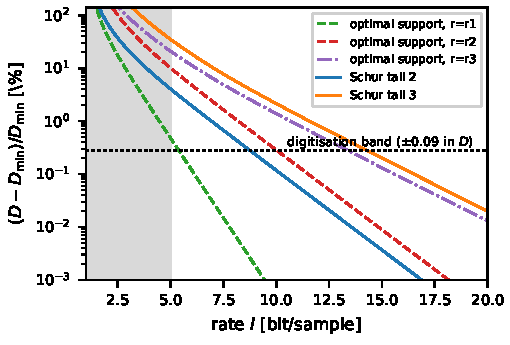
\includegraphics[width=\columnwidth]{fig_wall.pdf}
 \caption{The wall as a horizontal asymptote, for the five families of
 Table~\ref{tab:wall}. The shaded band is the published abscissa range
 $I\in[1,5]$; the dashed line is the digitisation floor
 $\pm0.09$ expressed relative to the lowest wall in the table ($0.28\%$). No
 family has entered that floor inside the published window --- the closest,
 the $r=1$ optimal support, is still $0.21$ units above its wall at $I=5$.}
 \label{fig:wall}
\end{figure}

\begin{corollary}[the published figure does not show a wall]
\label{cor:noshows}
The published figure is drawn on $D\in[40,90]$, $I\in[1,5]$. By
Proposition~\ref{pr:region}(i) a wall becomes visible only where the frontier is
within digitisation of $D_{\min}$: measured on the ray, $V=\operatorname{range}(F_2^{\top})$
first enters $\pm0.09$ of its wall at $I=9.3$, and the fastest of the five
families of Table~\ref{tab:wall} does so at $I=5.6$ --- both outside the
published abscissa range, so \emph{no} family in that table can display its wall
there. The left end of the red curve is $(D,I)=(46.99,\,4.921)$, and $4.921$ is
the top frame edge minus one line width: the red curve is truncated by the
\emph{top} edge, and its terminal abscissa carries no information about
$D_{\min}(V)$; numerically $46.99-D_{\min}=+0.87$, far outside the calibration
band. The blue and magenta curves end at $D=40.08$, i.e.\ they are truncated by
the \emph{left} edge, at rates $I=3.498$ and $3.263$, while their walls lie
below the axis: for the unrestricted magenta curve the wall is exactly
$j_c=31.4833$ (full rank, so the zero-noise limit is the exact-observation
limit), and for the blue curve even the lowest wall it could be assigned, the
$r=3$ optimal support at $31.6420$, sits $8.4$ units under the frame edge.
\end{corollary}

Fig.~\ref{fig:wall} is therefore drawn on axes that reach $I=20$ rather than by
annotating the published window: on the published window the phenomenon of
Corollary~\ref{cor:noshows} is not visible, only its absence is.


\section{The floor does not order the frontier}
\label{sec:nofactor}

Because $D_{\min}(V)$ depends on $S$ only through $\operatorname{range}(S)$ ---
the shape of the spectrum does not enter it, confirmed by scanning anisotropic
spectra within a fixed subspace --- it is tempting to summarise the design
problem as ``pick the subspace by the wall, pick the spectrum by the rate''.
The following counterexample says the second half is not free.

\begin{proposition}[non-factorisation]
\label{pr:nofactor}
There exist unit directions $z_1,z_2\in\mathbb R^{4}$ with
\[
 \big|\Phi_0(z_1z_1^{\top})-\Phi_0(z_2z_2^{\top})\big|
 \big/\max_i\Phi_0(z_iz_i^{\top}) = 1.46\times10^{-3}
\]
but frontier values differing by $45\%$ at a fixed rate:
$D_{I=2}=1108.36$ versus $1610.70$, and by $13.7\%$ at $I=3$ ($727.39$ versus
$826.95$). Hence no function of the wall alone determines the frontier.
\end{proposition}

\begin{table}[h]
 \centering\caption{Rank-one directions: wall pairing versus frontier
 ordering.}
 \label{tab:nofactor}
 \begin{tabularx}{\columnwidth}{Xl}
 \hline
 wall ratio $<5\times10^{-3}$ & 1 pair; rate spread at $I=2$: $45.3\%$ \\
 wall ratio $<10^{-3}$ & no pair \\
 \emph{inverted pairs} & $111$ at $I=2$, $31$ at $I=3$ \\
 spread of $D_{I=2}$ within deciles & $53\%$--$1.8\times10^{4}\%$, none $<50\%$ \\
 \hline
 \end{tabularx}
 \\[1pt]{\scriptsize $120$ draws (\texttt{rng(5)}), $76$ admissible; walls from
 the zero-noise fixed point, frontiers from a $20$-step ray bisection using the
 information-form recursion only (no DARE solve, no spectral-radius test).
 ``Inverted pairs'': higher wall but lower cost at equal rate.}
\end{table}

The robust statement is the count of inverted pairs, not the single $45\%$
pair: a tolerance-based pairing can vanish when the tolerance is tightened, but
$111$ inversions of the wall ordering do not. What survives, and what we assert,
is the exact factorisation statement plus its restriction:
\begin{itemize}
 \item $\Phi_0$ is a function of $\operatorname{range}(S)$ alone
;
 \item the frontier is \emph{not} monotone in $\Phi_0$, even within the rank-one
 family;
 \item consequently the two design coordinates (wall, rate) decouple only
 \emph{within} a fixed subspace, not \emph{across} subspaces.
\end{itemize}


\section{Limitations: what this note does not claim}
\begin{itemize}
 \item All rate-side numbers are \emph{constructive upper bounds} obtained by
 local descent over the cone. Section~\ref{sec:waterfill} adds a
 closed-form lower bound, proved only at a frozen prior; its frontier-wide
 form needs a monotonicity that \emph{fails} (a closed-form rank-one
 counterexample and $115$ reachable in-cone counterexamples), so the
 frontier-wide bound is not claimed at all; it leaves
 $2.7$--$4.5$ units of $D$ uncertified at $I=3$ and $11$--$15$ at $I=2$,
 and it does not certify the published blue point infeasible
 (Section~\ref{sec:waterfill},).
 \item Every quantitative statement is for the published four-state example;
 the subspace-selection phenomena are not claimed to hold for a general
 plant, and the general statement is left to the follow-up on the dynamic
 minimal stage.
 \item The blue curve of the published figure is not reproduced
 (Remark~\ref{rmk:blue}).
 \item The rank-one global optimality of the wall-side rule is supported by
 repeated descent runs and by a two-valued landscape
 ($10.169224$ / $86.665888$), not by a proof; the descent reports the
 best of several starts and is not certified to hit the global minimum on
 every run.
\end{itemize}
